%\section{Drone movement}\label{s:drone_movement}
In order to make a transfer function for the drone it is needed to examine how the drone behaves, when it moves around. To make it simple the drone is set to only move in z-axis also known as yaw axis \ref{fig:z_axis}.
\begin{figure}[H]
    \centering
    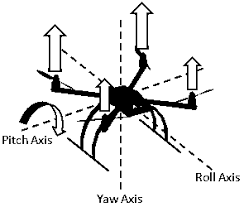
\includegraphics[width=0.45\textwidth]{figures/ch_movement/z-axis.png}
    \caption{Illustration of a drone in 3D-plane \cite{drone_axis}.}
    \label{fig:z_axis}
\end{figure}

 As mentioned in the requirement specification \ref{sec:req}, the drone should keep a fixed distance to the floor. To be able to control the drone in the z-axis, a model for the drone will be determined. This model describing how the drone corresponds to controller inputs. The position on the z-axis is controlled by the throttle on the remote controller. The throttle values is set from 1000\% - 2000\%, where the drone is idle at 1000\% and maximum velocity at 2000\%.  

\section{Vicon}\label{s:vicon}
To determine the behaviour of the drone, it is important to know how the the drone response to the remote controller. 
Since the control system of the flight controller is unfamiliar, it will be difficult to determine the model for the drone precisely by calculations. An alternative way is by measuring the step response or impulse response in z-axis in an exploratory method. The step response has been chosen rather than the impulse response, since it is easier to measure and more accurate measurements. For measuring the response, the chosen flight controller combined with position sensors or a motion tracker system will be used. The motion tracker system is called Vicon, which is available at Aalborg university, in the motion tracking laboratory. The Vicon system is able to detect the drone position over time within millimeter accuracy, which is possible by the use of Vicon cameras \cite{Vicon}.

For measuring the step response, the Vicon system will be used, because of the indoor position tracking possibilities.


\section{Transfer function for the movements}\label{s:transfer_function}
To make the model of the drone's movement, it is first needed to find a transfer function to describe the movements. To get the data for the transfer function, a step response is made with the drone, to track the drone in the step response, the Vicon system is used. Because the model only has to cover the z-axis, the step response will only be made for this axis. From the step response a transfer function can be found. This function is called $G(s)$. 
The control loop has feedback from the sensor. The system can be seen on figure \ref{fig:transfer_function}.
%that depends on the input and output of the function. All these functions depends on the time. To get a better view of have this transfer function works can be seen on the figure \ref{fig:transfer_function}.
\begin{figure}[H]
    \centering
    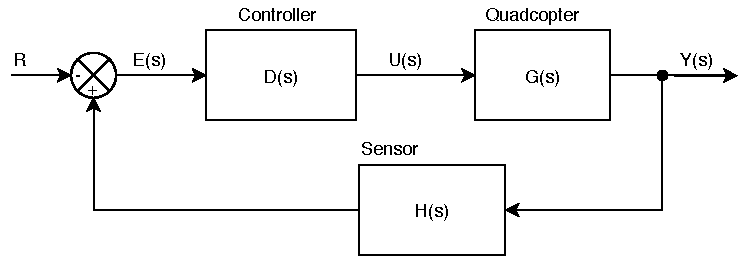
\includegraphics[width=0.75\textwidth]{figures/ch_design/transfer_function.pdf}
    \caption{An illustration of the transfer diagram.}
    \label{fig:transfer_function}
\end{figure}

\subsection*{Flight measuring test}
For getting the step response, a test have been made in the motion tracking Lab (MT-lab). The test was executed by setting the thrust to 33\% in 1 second to simulate a step. The results are shown on the graph in figure \ref{fig:results_mesuring_test_drone}.
\begin{figure}[h]
    \centering
    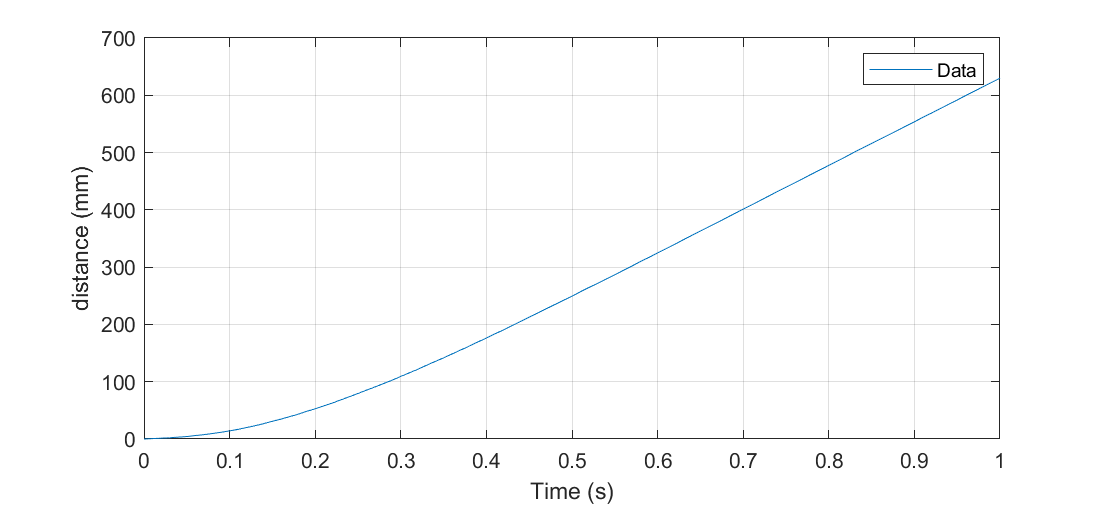
\includegraphics[width=0.8\textwidth]{figures/Appendix/measuringTest/DroneTest.png}
    \caption{Graph showing the results of the flight measuring test in a appendix \ref{ap:drone_flight_test}.}
    \label{fig:results_mesuring_test_drone}
\end{figure}
\newline
With the results from figure \ref{fig:results_mesuring_test_drone}, the velocity over time can be found, which can be seen in figure \ref{fig:DroneVelocity}.
\begin{figure}[h]
    \centering
    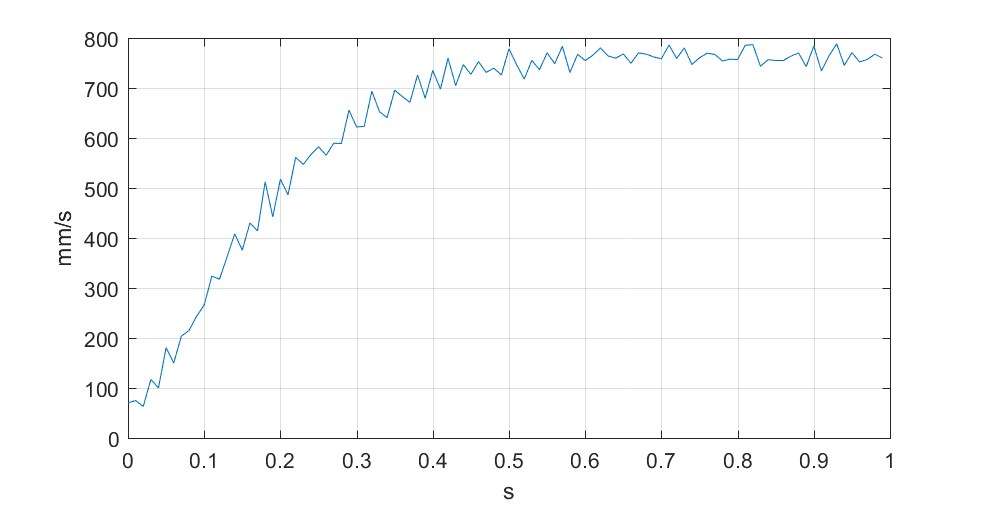
\includegraphics[width=0.8\textwidth]{figures/ch_movement/velocityDrone.png}
    \caption{Change of the velocity over 1 second with the qaudcoptors thrust set to 33\%.}
    \label{fig:DroneVelocity}
\end{figure}
\newline
This data can be used for making the transfer function for the control loop. From the data it have been chosen to estimate for a first order transfer function. 

\subsection*{Determination of the first order transfer function}
A first order system has the function given by equation \ref{eq:firstOrderSystem} \cite{Bolton2002}.
\begin{equation}\label{eq:firstOrderSystem}
    G(s)=\frac{K}{\tau s + 1}
\end{equation}
Where $K$ is the steady-state gain and $\tau$ is the time constant. 
The stationary gain can be observed from the graph on figure \ref{fig:DroneVelocity}, and are observed to be 770. 
The time constant is found at 63\% of the steady-state gain, where the value at 63\% of 770 mm/s is 485.1 mm/s. 
The time constant is read from the graph to 0.20 second \cite{Bolton2002}.
With the stationary gain and the time constant are found, the transfer function can be defined as equation \ref{eq:transferFunktionOfDrone}.
\begin{equation}\label{eq:transferFunktionOfDrone}
    G(s)=\frac{770}{0.2 s + 1}
\end{equation}
A simulation of the determined transfer function compared to the velocity can be seen in figure \ref{fig:Deter_transfor_function} 
\begin{figure}[h]
    \centering
    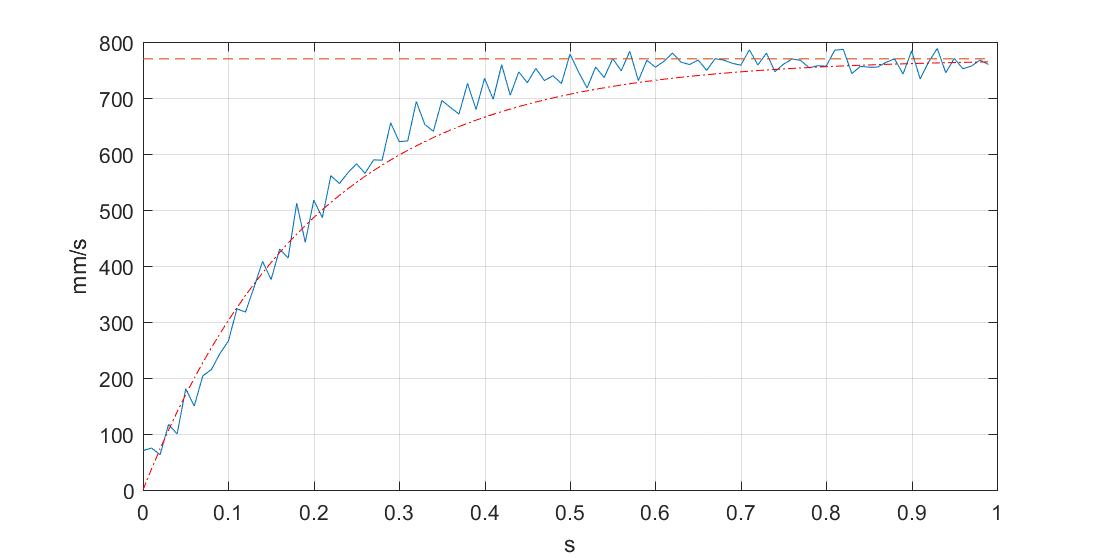
\includegraphics[width=0.8\textwidth]{figures/ch_movement/TransferFuntionDrone.png}
    \caption{Graph of the found transfer function compered to the measured velocity of the drone for 1 second. Where the continuous line are the Velocity, the dashed line are final value and the dash-dot line are the transfer function.}
    \label{fig:Deter_transfor_function}
\end{figure}
\newline
As the output of the transfer function is the height, the integrator $\frac{1}{s}$ is applied. $G(s)$ this gives the function in equation \ref{eq:finalTranforfunktionDrone}.
\begin{equation}\label{eq:finalTranforfunktionDrone}
    G(s) = \frac{770}{0.2 s+1}\cdot \frac{1}{s}
\end{equation}